\chapter{Planeación de movimientos}
Una de las capacidades base que se busca que tenga el robot al deber colaborar con otros equipos mecánicos y estaciones de trabajo donde los elementos cuentan con posiciones específicas es la posibilidad de moverse evitando colisiones con dichos elementos y al mismo tiempo, que el efector final logre obtener las posiciones requeridas para llevar a acabo la actividad que se le solicita. Para esto es necesario realizar el estudio de la construcción mecánica del robot, de tal forma de se calculen las fuerzas que se deben aplicar en cada actuador perteneciente a la estructura del manipulador, mediante los análisis \textbf{cinemáticos y dinámicos} del robot.

Esta definición de la posición del robot en función del tiempo se conoce como \textbf{trayectoria}\cite{lynch_modern_2017}. En Robótica, cada punto en el espacio de trabajo corresponde a una configuración única de los actuadores del robot y cada una de estas configuraciones se puede representar como un punto en un espacio conformado por el conjunto de configuraciones posibles de acuerdo con la configuración física del robot. De esta manera, la configuración de un brazo robótico con $n$ articulaciones se puede representar como una lista de $n$ posiciones articulares: $q = (\theta_{0},...,\theta_{n})$. Siguiendo las condiciones anteriores, los autores definen el \textit{espacio de configuraciones libre} como aquel que contiene todas las configuraciones del robot en las que no colisiona con ningún obstáculo ni excede los límites de sus articulaciones \cite{lynch_modern_2017}.

Dentro del trabajo realizado se busca que el robot sea capaz de dirigir su efector final a la coordenada en que se estima se encuentre la pieza de interés. Una vez que se ha conectado este objetivo específico con los conceptos teóricos anteriormente mencionados, es posible remarcar el uso de la \textbf{Cinemática directa}, la cual se encarga del cálculo de la posición y orientación de un sistema coordenado asociado al efector final del robot desde las coordenadas $\theta$ de sus articulaciones \cite{lynch_modern_2017} 

La implementación de este análisis se realizó utilizando la herramienta MoveIt, que es posible utilizar dentro del entorno de ROS. esta herramienta lleva a cabo los cálculos necesarios para obtener los movimientos necesarios en la configuración del manipulador para alcanzar una pose específica. 

\section{Movimiento de cuerpo rígido}

\subsection{Posición y Orientación}
De acuerdo con Asada y Slotine en \cite{asada_robot_1986}, la estructura formada por un manipulador puede ser modelada por medio de cuerpos rígidos. Adicionalmente, Gross et al. (2013)\cite{gross_statics_2013} definen el cuerpo rígido como aquel que no se deforma bajo la influencia de fuerzas, es decir, que las distancias entre diferentes puntos del cuerpo se mantienen constantes.

Los autores también comentan que para describir completamente la localización de un cuerpo rígido dentro del espacio es necesario conocer su posición y su orientación. Para conocer la posición, es necesario que exista un punto de referencia, fijo, y un sistema de coordenadas asociado al mismo, a partir del cual se tomarán las distancias que describen la posición relativa del punto que representa el punto de interés con respecto a la referencia. Convencionalmente, el sistema de referencia utilizado es aquel construido con los vectores unitarios \textit{(i,j,k)}, estos vectores dictan la dirección de los ejes \textit{(X,Y,Z)} con los cuales se define un espacio tridimensional. De esta forma, se utilizan las distancias sobre estos ejes que definen la relación entre dos puntos del espacio, en este caso, el cuerpo rígido y el origen el sistema. 

Además de las distancias, es posible establecer las relaciones angulares que definen la relación entre el origen del sistema y el cuerpo de estudio, siendo posible una inclinación en cualquiera de estos ejes de forma independiente o bien, una combinación de rotaciones en todos ellos. 

La posición del cuerpo rígido puede representarse matemáticamente utilizando un vector compuesto por las tres distancias que definen su relación con el sistema de referencia de la siguiente manera: $P_{0} = (x_{0},y_{0}, z_{0})$.

De forma similar, en \cite{asada_robot_1986} los autores comentan que para representar la orientación de un cuerpo rígido, se definen tres ejes coordenados esta vez asociados al cuerpo rígido, en la figura \ref{fig:RigidBodyPos} el origen de este segundo sistema coordenado se encuentra señalizado como $O_{1}$, y los ejes como $(X_{1},Y_{1},Z_{1})$. Este nuevo sistema se encuentra conectado al cuerpo rígido y se mueve junto a él. 

\begin{figure}[ht]
\centering
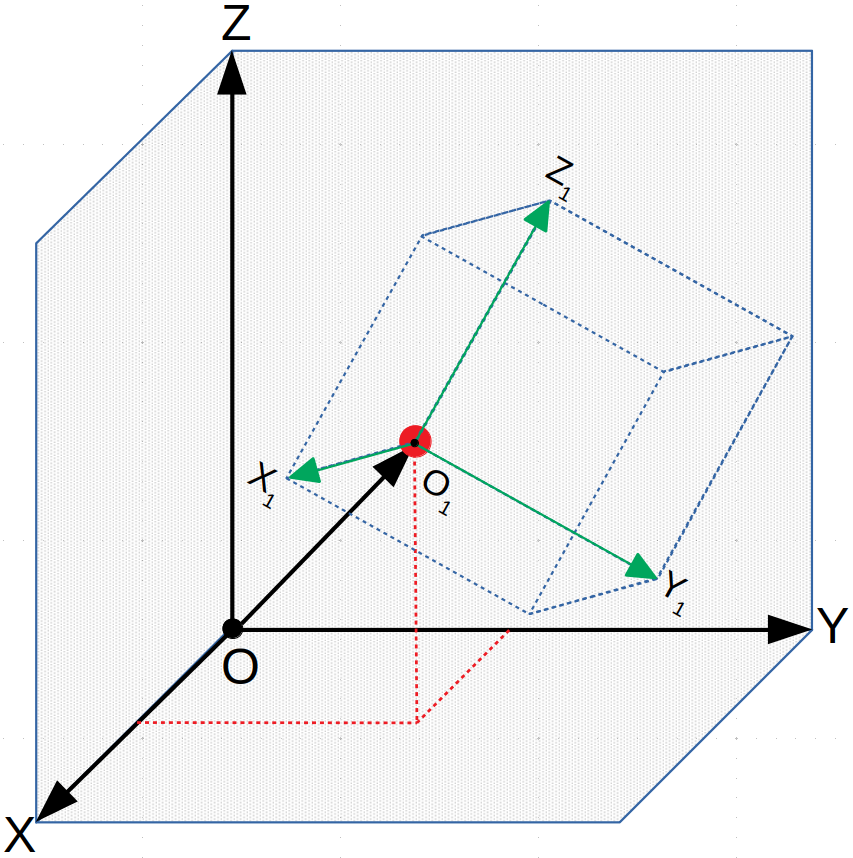
\includegraphics[scale= 0.2]{Figures/RigidBodyPos.png}
    \caption{Posición y Orientación de un cuerpo rígido}
    \label{fig:RigidBodyPos}
\end{figure}

Para el estudio de la orientación entre los sistemas coordenados establecidos es pertinente mencionar el concepto de las rotaciones básicas. En \cite{olguin_diaz_3d_2019} Olguín explica que una simplificación útil para este planteamiento es considerar un movimiento rotatorio sin traslación. Si se considera únicamente la rotación sobre uno de los ejes Cartesianos se conoce como una Rotación Básica. El autor añade en su explicación las matrices asociadas a las rotaciones sobre los ejes. Utilizando estas matrices es posible encontrar la posición de un punto existente en el sistema rotado, mediante la transformación que resulta en sus coordenadas referentes al sistema original.

\begin{equation*}
    R_{x,\phi}=\begin{bmatrix}
    1 & 0 & 0\\
    0 & cos_{\phi} & -sin_{\phi}\\
    0 & sin_{\phi} & cos_{\phi}
    \end{bmatrix}
\end{equation*}

\begin{equation*}
    R_{y,\theta}=\begin{bmatrix}
    cos_{\theta} & 0 & sin_{\theta}\\
    0 & 1 & 0\\
    -sin_{\theta} & 0 & cos_{\theta}\\
    \end{bmatrix}
\end{equation*}

\begin{equation*}
    R_{z,\psi}=\begin{bmatrix}
    cos_{\psi} & -sin_{\psi} & 0\\
    sin_{\psi} & cos_{\psi} & 0\\
    0 & 0 & 1
    \end{bmatrix}
\end{equation*}

Como parte del análisis del movimiento del robot comúnmente se encuentran rotaciones que no coinciden con el movimiento sobre solo uno de los ejes, sino que se tratan de movimientos complejos que resultan de combinaciones de otros movimientos. En \cite{olguin_diaz_3d_2019} los autores establecen que toda rotación se obtiene con rotaciones básicas sucesivas. Sin embargo, consideran importante apuntar que es indispensable conocer el orden en el cual se realizan las rotaciones, dado que rotaciones sobre el sistema original (extrínsecas) dan resultados distintos que las rotaciones realizadas sobre el sistema coordenado asociado al cuerpo rígido (intrínsecas), este planteamiento permite la existencia de diferentes combinaciones de secuencias de rotación que llevan al mismo resultado. Para esto, Olgín menciona el estudio de \textbf{Rotaciones Compuestas}, con el cual es posible analizar las interacciones entre las diferentes matrices de rotación y su efecto en el objeto. Dentro de la notación utilizada para este tema es común encontrar lo siguiente: \textbf{$R_{a}^{b}$} y \textbf{$p^{(a)}$}, la primera expresión se refiere a la rotación existente entre el sistema \textbf{$b$} usando como referencia al sistema \textbf{$a$} y la segunda al punto \textbf{$p$} usando como origen al sistema \textbf{$a$}. Utilizando esta notación se puede expresar la relación entre el punto y las matrices de rotación.
Asumiendo la existencia de los sistemas coordenados $\Sigma_{0}$, $\Sigma_{1}$ y $\Sigma_{2}$, la orientación de un punto $p$ se puede expresar de la siguiente forma: 

\begin{equation*}
    p^{(1)}=R_{1}^{2}p^{(2)}
\end{equation*}
\begin{equation*}
    p^{(0)}=R_{0}^{1}p^{(1)} =R_{0}^{1}R_{1}^{2}p^{(2)} =R_{0}^{2}p^{(2)}
\end{equation*}

En las ecuaciones anteriores se puede observar una de las propiedades del análisis de las matrices de rotación. En este caso, la matriz de rotación compuesta $R_{0}^{2}$ se puede obtener mediante una multiplicación matricial para rotaciones intrínsecas:

\begin{equation*} R_{0}^{2}=R_{0}^{1}R_{1}^{2}
\end{equation*}

\emph{Ángulos de Euler}

Una vez que se ha establecido como base el análisis de las rotaciones, en \cite{olguin_diaz_3d_2019} el autor indica que \textit{-toda combinación de rotaciones básicas sobre los ejes principales tiene tres ángulos \textbf{independientes} conocidos como los Ángulos de Euler-}, profundiza diciendo que las rotaciones básicas pueden realizarse ya sea todas en el sistema coordenado base (parametrización extrínseca), todas en el sistema coordenado actual (parametrización intrínseca), o bien usando una combinación de las posibilidades anteriores. Esta última opción conlleva procedimientos muy engorrosos, por lo que el autor no recomienda su uso. Olguín indica también que en la práctica hay 24 formas distintas de representar una matriz de rotación utilizando 3 ángulos de Euler independientes, conformadas de 12 combinaciones extrínsecas para rotaciones basadas en un sistema coordenado fijo y 12 combinaciones intrínsecas para rotaciones basadas en el sistema coordenado actual.

\emph{Cuaterniones}\\
La representación de la orientación por medio de cuaterniones fue planteada inicialmente por Sir William Rowan Hamilton \cite{hamilton_ii_1844} y se utiliza en robótica gracias a que no se obtienen singularidades, como sí sucede con la representación con Ángulos de Euler o Ángulos fijos. También se considera imprescindible mencionarlos dado que el middleware ROS, utilizado durante la implementación de este proyecto recurre a ellos para las transformaciones homogéneas que realiza.
De acuerdo con Siciliano, B. \& Khatib, O. (Eds.). (2016) \cite{siciliano_springer_2016}, un cuarternion \textbf{$\epsilon$} se define de la siguiente forma:
\begin{equation*}
    \epsilon = \epsilon_{0}+\epsilon_{1}i+
    \epsilon_{2}j+
    \epsilon_{3}k
\end{equation*}

En la ecuación anterior, los componentes $\epsilon_{0}$, $\epsilon_{1}$, $\epsilon_{2}$ y $\epsilon_{3}$, son escalares, conocidos en ocasiones como parámetros de Euler, mientras que $i$, $j$ y $k$ son operadores y se definen para satisfacer las siguientes reglas de correspondencia.

\begin{equation*}
    ii=jj=kk=-1
\end{equation*}
\begin{equation*}
    ij=k,\quad jk=i, \quad ki=j
\end{equation*}
\begin{equation*}
    ji=-k, \quad kj = -i, \quad ik = -j
\end{equation*}

Continuando con la descripción de los editores, mencionan elementos matemáticos necesarios para el manejo algebráico de los cuaterniones.

\textbf{Suma de cuaterniones}: se obtiene al sumar por separado sus respectivos componentes:\\
\begin{equation*}
    \epsilon_{A} = \epsilon_{0}+\epsilon_{1}i+
    \epsilon_{2}j+
    \epsilon_{3}k
\end{equation*}

\begin{equation*}
    \epsilon_{B} = \epsilon_{4}+\epsilon_{5}i+
    \epsilon_{6}j+
    \epsilon_{7}k
\end{equation*}

\begin{equation*}
    \epsilon_{C} = \epsilon_{A} + \epsilon_{B}
\end{equation*}
\begin{equation*}
\epsilon_{C} =                     (\epsilon_{0}+
    \epsilon_{4})+(\epsilon_{1}+\epsilon_{5})i+
    (\epsilon_{2}+\epsilon_{6})j+
    (\epsilon_{3}+\epsilon_{7})k
\end{equation*}

\textbf{Elemento nulo para adición}

\begin{equation*}
    0 = 0 + 0i + 0j + 0k
\end{equation*}

\textbf{Elemento nulo para multiplicación}

\begin{equation*}
    I = 1 + 0i + 0j + 0k
\end{equation*}

Comúnmente, el elemento $\epsilon_{0}$ es conocido como la parte escalas del cuaternion, mientras que los elementos $(\epsilon_{1},\epsilon_{2}, \epsilon_{3})$ se conoce como la parte vectorial.

\section{Transformaciones homogéneas}

El uso de Matrices de Transformaciones Homogéneas en el análisis del movimiento, tanto de cuerpos rígidos como su aplicación en robótica, permite el manejo matemático de la orientación y la posición del cuerpo rígido en un espacio tridimensional, estas son matrices de $4 \times 4$ y cumplen con la siguiente forma:\\

\begin{equation*}
	T = 
    \begin{bmatrix}
	R & p\\
	0 & 1 
	\end{bmatrix} = 
    \begin{bmatrix}
	r_{11} & r_{12} & r_{13} & p_{1}\\
	r_{21} & r_{22} & r_{23} & p_{2}\\
	r_{31} & r_{32} & r_{33} & p_{3}\\
	0 & 0 & 0 & 1 
	\end{bmatrix}
\end{equation*}

En \cite{lynch_modern_2017} se listan a manera de Proposiciones algunas de las propiedades de las matrices de transformación homogéneas, como son:\\
\begin{itemize}
    \item La inversa de una matriz de Transformación $T \in SE(3)$ es también una matriz de transformación y cumple con la siguiente forma:
    \begin{equation*}
        T^{-1} = 
    \begin{bmatrix}
	R & p\\
	0 & 1 
	\end{bmatrix}^{-1} = 
    \begin{bmatrix}
	R^{T} & -R^{T}p\\
	0 & 1 
	\end{bmatrix}
    \end{equation*}
    \item El producto de dos matrices de transformación es también una matriz de transformación.
    \item La multiplicación de matrices de transformación cumple con la propiedad asociativa: $(T_{1}T_{2})T_{3}=T_{1}(T_{2}T_{3})$, pero no con la propiedad conmutativa: $T_{1}T_{2}\neq T_{2}T_{1}$  
\end{itemize}

Siguiendo la descripción del autor en \cite{lynch_modern_2017}, es útil calcular el valor de $Rx+p$, siendo que $x \in R^{3}$ y $(R,p)$ representa la matriz $T$. Para hacer compatible el vector $x$ con las dimensiones de la matriz $T$, se concatena un $1$ al vector $x$, con lo cual es posible realizar el cálculo mediante una multiplicación de matrices.

\begin{equation*}
    T \begin{bmatrix}
        x\\1
    \end{bmatrix} = 
    \begin{bmatrix}
	R & p\\
	0 & 1 
	\end{bmatrix}
    \begin{bmatrix}
	x\\
	1 
	\end{bmatrix}=
    \begin{bmatrix}
	Rx + p\\
    1 
	\end{bmatrix}
\end{equation*}

De esta operación se obtiene el vector $ \left[x^{T}\quad 1\right]^{T}$ se conoce como la representación de $x$ en coordenadas homogéneas. En el contexto en que no encontramos, estas matrices son comúnmente utilizadas para cambiar los sistemas coordenados que se utilizan como referencia. 

De forma similar a las matrices de Rotación mencionadas anteriormente, la multiplicación de estas matrices permite obtener relaciones entre los distintos sistemas de referencia:

\begin{equation*}
    T_{ab}T_{bc} = T_{a\cancel{b}}T_{\cancel{b}c}=T_{ac}
\end{equation*}

\begin{equation*}
    T_{ab}v_{b} = T_{a\cancel{b}}v_{\cancel{b}}=v_{a}
\end{equation*}

\section{Descripción cinemática del robot}

La estructura que compone al robot para la implementación de este proyecto se muestra en la figura \ref{fig:Robotino_models}, donde se observan dos perspectivas del robot utilizando la interfaz gráfica Rviz. Para este despliegue, se cuenta con los modelos de los sensores Kinect, Hokuyo, la base del robot y la plataforma. Los elementos adicionales se representan mediante figuras tridimensionales, cuyas medidas corresponden con las de los elementos reales del robot.

\begin{figure}[H]
    \centering
    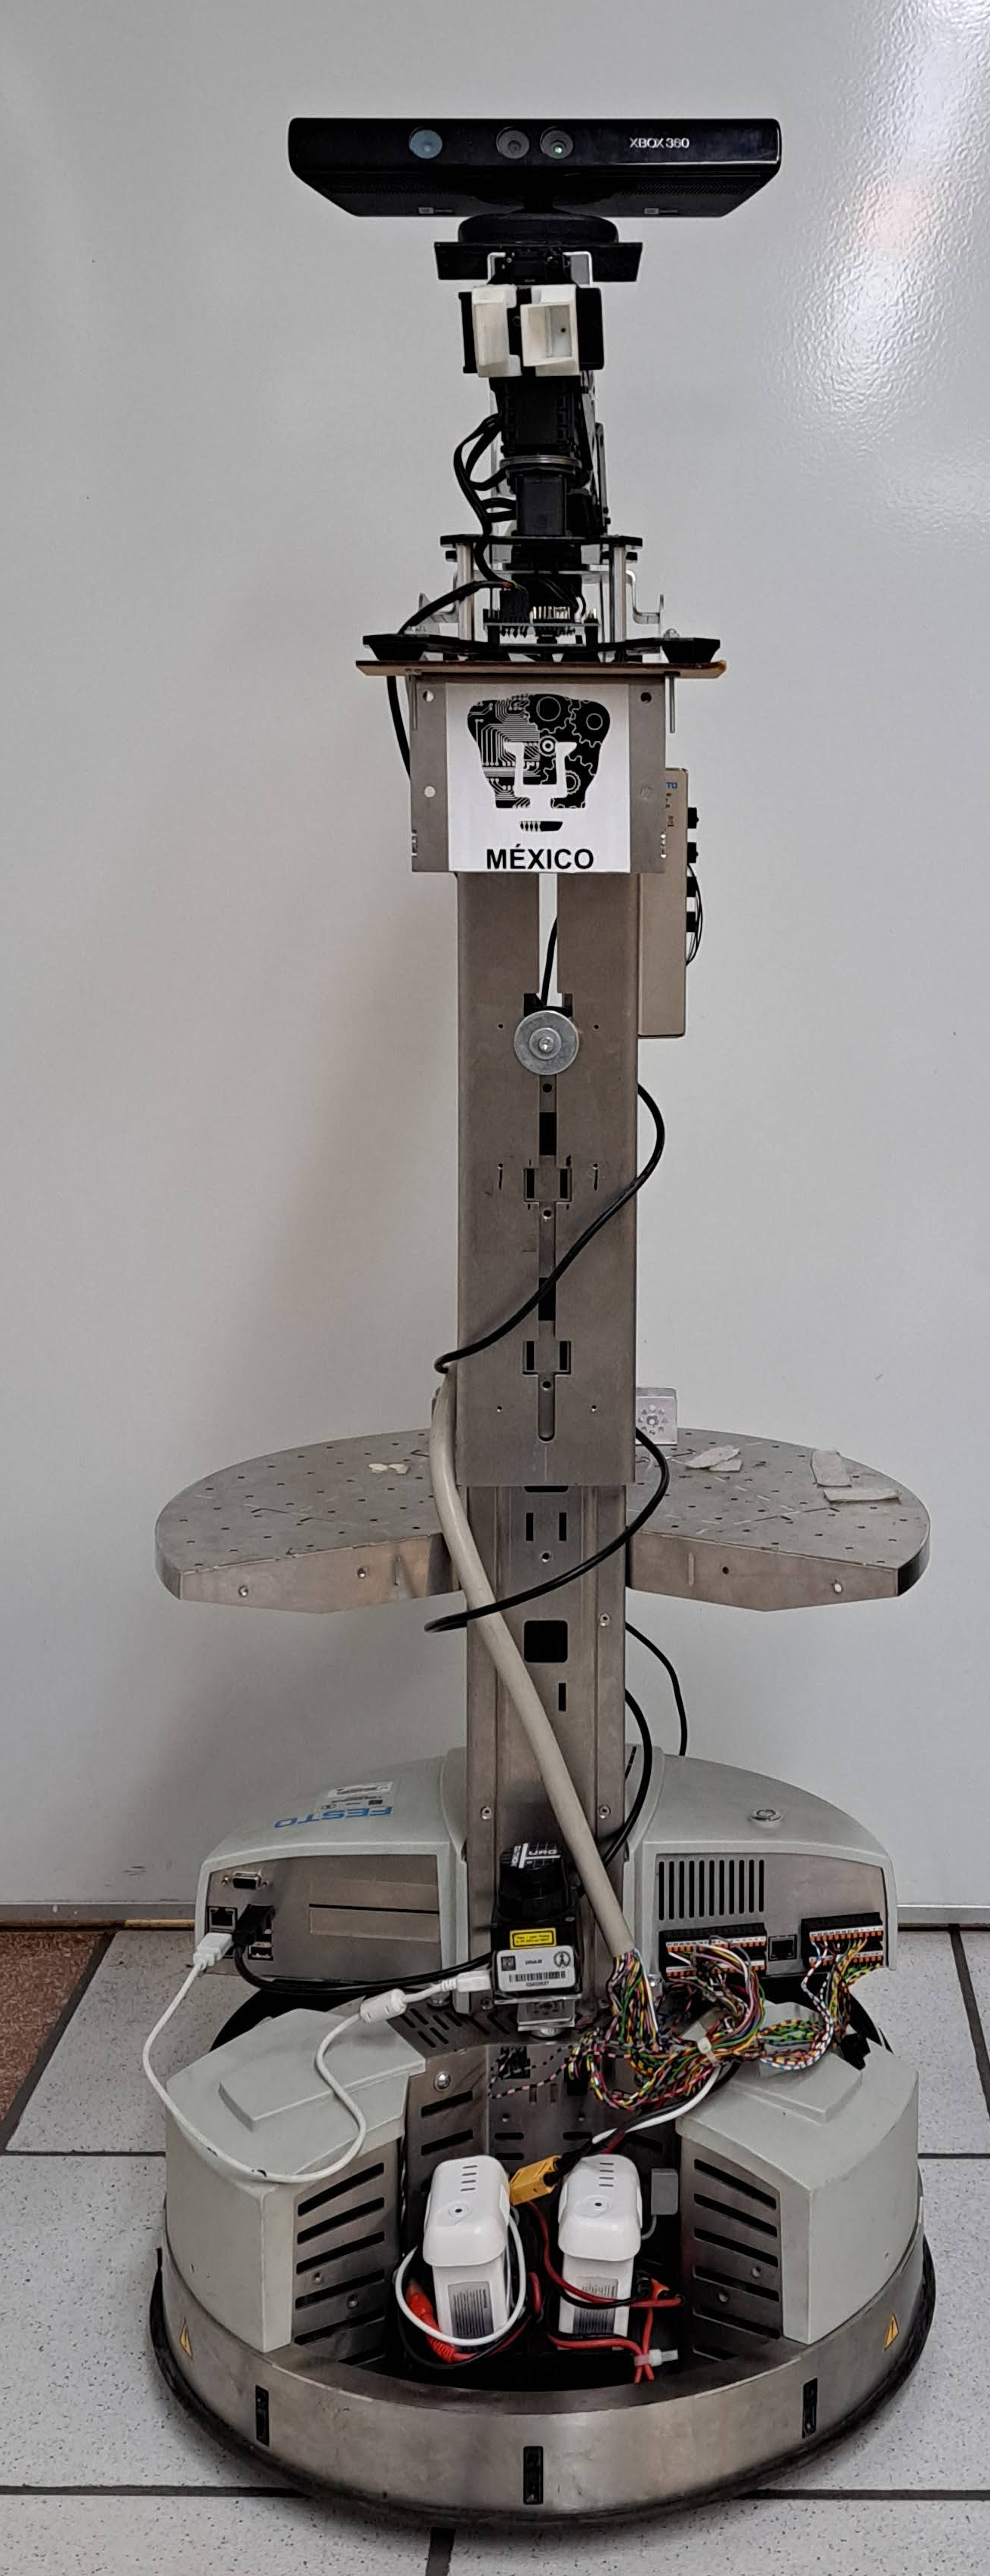
\includegraphics[scale=0.4]{Figures/Robotino_New_New.png}   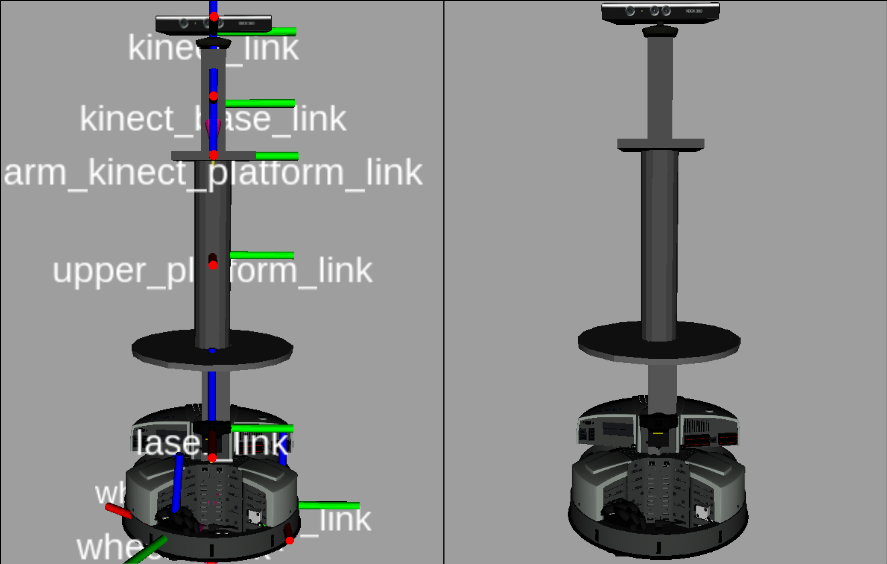
\includegraphics[scale=0.4]{Figures/Robotino_model_front.png}
    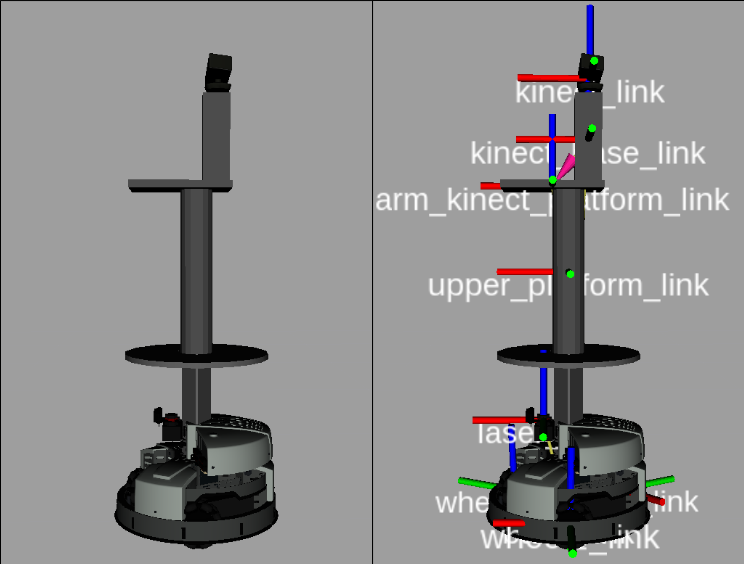
\includegraphics[scale=0.4]{Figures/Robotino_model_side.png} 
        \caption{Árbol cinemático del robot}
        \label{fig:Robotino_models}
\end{figure}

Todas las articulaciones del robot con la configuración utilizada para este proyecto son rotacionales.

\begin{figure}[H]
    \centering
    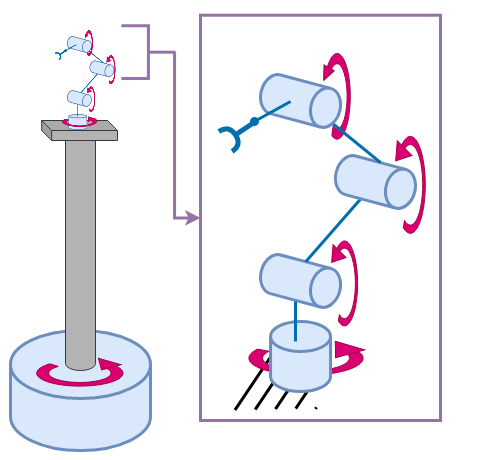
\includegraphics[scale=0.4]{Figures/Robotino_DescCin.png}
        \caption{Descripción cinemática}
        \label{fig:RobotinoDescCin}
\end{figure}

\section{Manipulación de objetos}

Como se menciona en el capítulo anterior, se estima la posición de la pieza de interés utilizando la información obtenida del procesamiento que se realiza a la imagen en conjunto con el análisis de la nube de puntos. Sin embargo, la posición calculada tiene como sistema de referencia aquel asociado a la cámara del sensor Kinect, por lo que es necesario realizar la transformación de esas coordenadas a unas asociadas a la base del manipulador del robot. Con este fin se utilizan las herramientas mencionadas anteriormente. Para esta implementación se utilizó la paquetería \textbf{tf}\cite{tf_ROS} incluida en la infraestructura del middleware ROS, que facilita estos cálculos en tiempo real, así como su visualización durante el desarrollo y la ejecución. Adicionalmente, el cálculo de la trayectoria final que ha de seguir el manipulador para que el efector final llegue a su destino se realizó por medio de la paquetería MoveIt.



